\chapter{Thiết kế hệ thống}

Chương này trình bày quá trình thiết kế hệ thống quản lý bãi giữ xe dựa trên các yêu cầu đã phân tích ở Chương~3. Nội dung bao gồm kiến trúc tổng thể của hệ thống, mô hình dữ liệu, từ điển dữ liệu, các sơ đồ tuần tự mô tả luồng xử lý nghiệp vụ và thiết kế giao diện người dùng. Những nội dung này là cơ sở cho việc triển khai hệ thống ở Chương~5.

% ==================================================
\section{Kiến trúc tổng thể}
% ==================================================

Hệ thống được xây dựng theo mô hình kiến trúc ba lớp (Three-Tier Architecture) nhằm tách biệt giao diện người dùng, xử lý nghiệp vụ và truy cập dữ liệu. Cách tổ chức này giúp mã nguồn dễ bảo trì, dễ kiểm thử và thuận lợi khi mở rộng thêm chức năng trong tương lai.

Kiến trúc hệ thống bao gồm ba lớp chính:

\begin{itemize}
    \item \textbf{Lớp giao diện (GUI):} Gồm các Form WinForms dùng để tương tác với người dùng. Lớp này chịu trách nhiệm nhận dữ liệu đầu vào và hiển thị kết quả.

    \item \textbf{Lớp nghiệp vụ (BLL):} Thực hiện xử lý các quy tắc nghiệp vụ như kiểm tra dữ liệu hợp lệ, tính phí gửi xe, kiểm tra vé tháng, xử lý thống kê doanh thu và điều phối transaction.

    \item \textbf{Lớp truy cập dữ liệu (DAL):} Thực hiện các thao tác với cơ sở dữ liệu SQL Server thông qua ADO.NET như truy vấn, thêm, sửa và cập nhật dữ liệu.
\end{itemize}

Luồng hoạt động của hệ thống được thực hiện như sau: người dùng thao tác trên giao diện, yêu cầu được gửi đến lớp BLL để xử lý nghiệp vụ. Nếu cần truy xuất dữ liệu, BLL sẽ gọi DAL. Kết quả sau cùng được trả lại giao diện để hiển thị cho người dùng.

% ==================================================
\section{Sơ đồ ERD}
% ==================================================

Từ kết quả phân tích yêu cầu ở Chương~3, cơ sở dữ liệu được thiết kế xoay quanh sáu thực thể chính:

\begin{itemize}
    \item \textbf{LoaiXe:} Quản lý thông tin các loại xe.
    \item \textbf{BangGia:} Lưu trữ mức giá áp dụng cho từng loại xe.
    \item \textbf{TheXe:} Quản lý thông tin thẻ xe được cấp phát.
    \item \textbf{KhachHang:} Lưu trữ thông tin khách hàng.
    \item \textbf{VeThang:} Quản lý thông tin đăng ký vé tháng.
    \item \textbf{LuotGui:} Lưu trữ thông tin các lượt gửi xe.
\end{itemize}

Các quan hệ giữa các thực thể được xây dựng nhằm phản ánh đúng nghiệp vụ thực tế của bãi giữ xe:

\begin{itemize}
    \item Một loại xe được áp dụng một hoặc nhiều mức giá.
    \item Một khách hàng có thể đăng ký nhiều vé tháng trong các giai đoạn khác nhau.
    \item Một thẻ xe tham gia nhiều lượt gửi khác nhau.
    \item Một lượt gửi gắn với một thẻ xe và một loại xe.
    \item Một vé tháng thuộc về một khách hàng và được liên kết với thẻ xe tương ứng.
\end{itemize}

Hình~\ref{fig:erd} mô tả mô hình thực thể - liên kết (Entity Relationship Diagram) của hệ thống.

\begin{figure}[htbp]
    \centering
    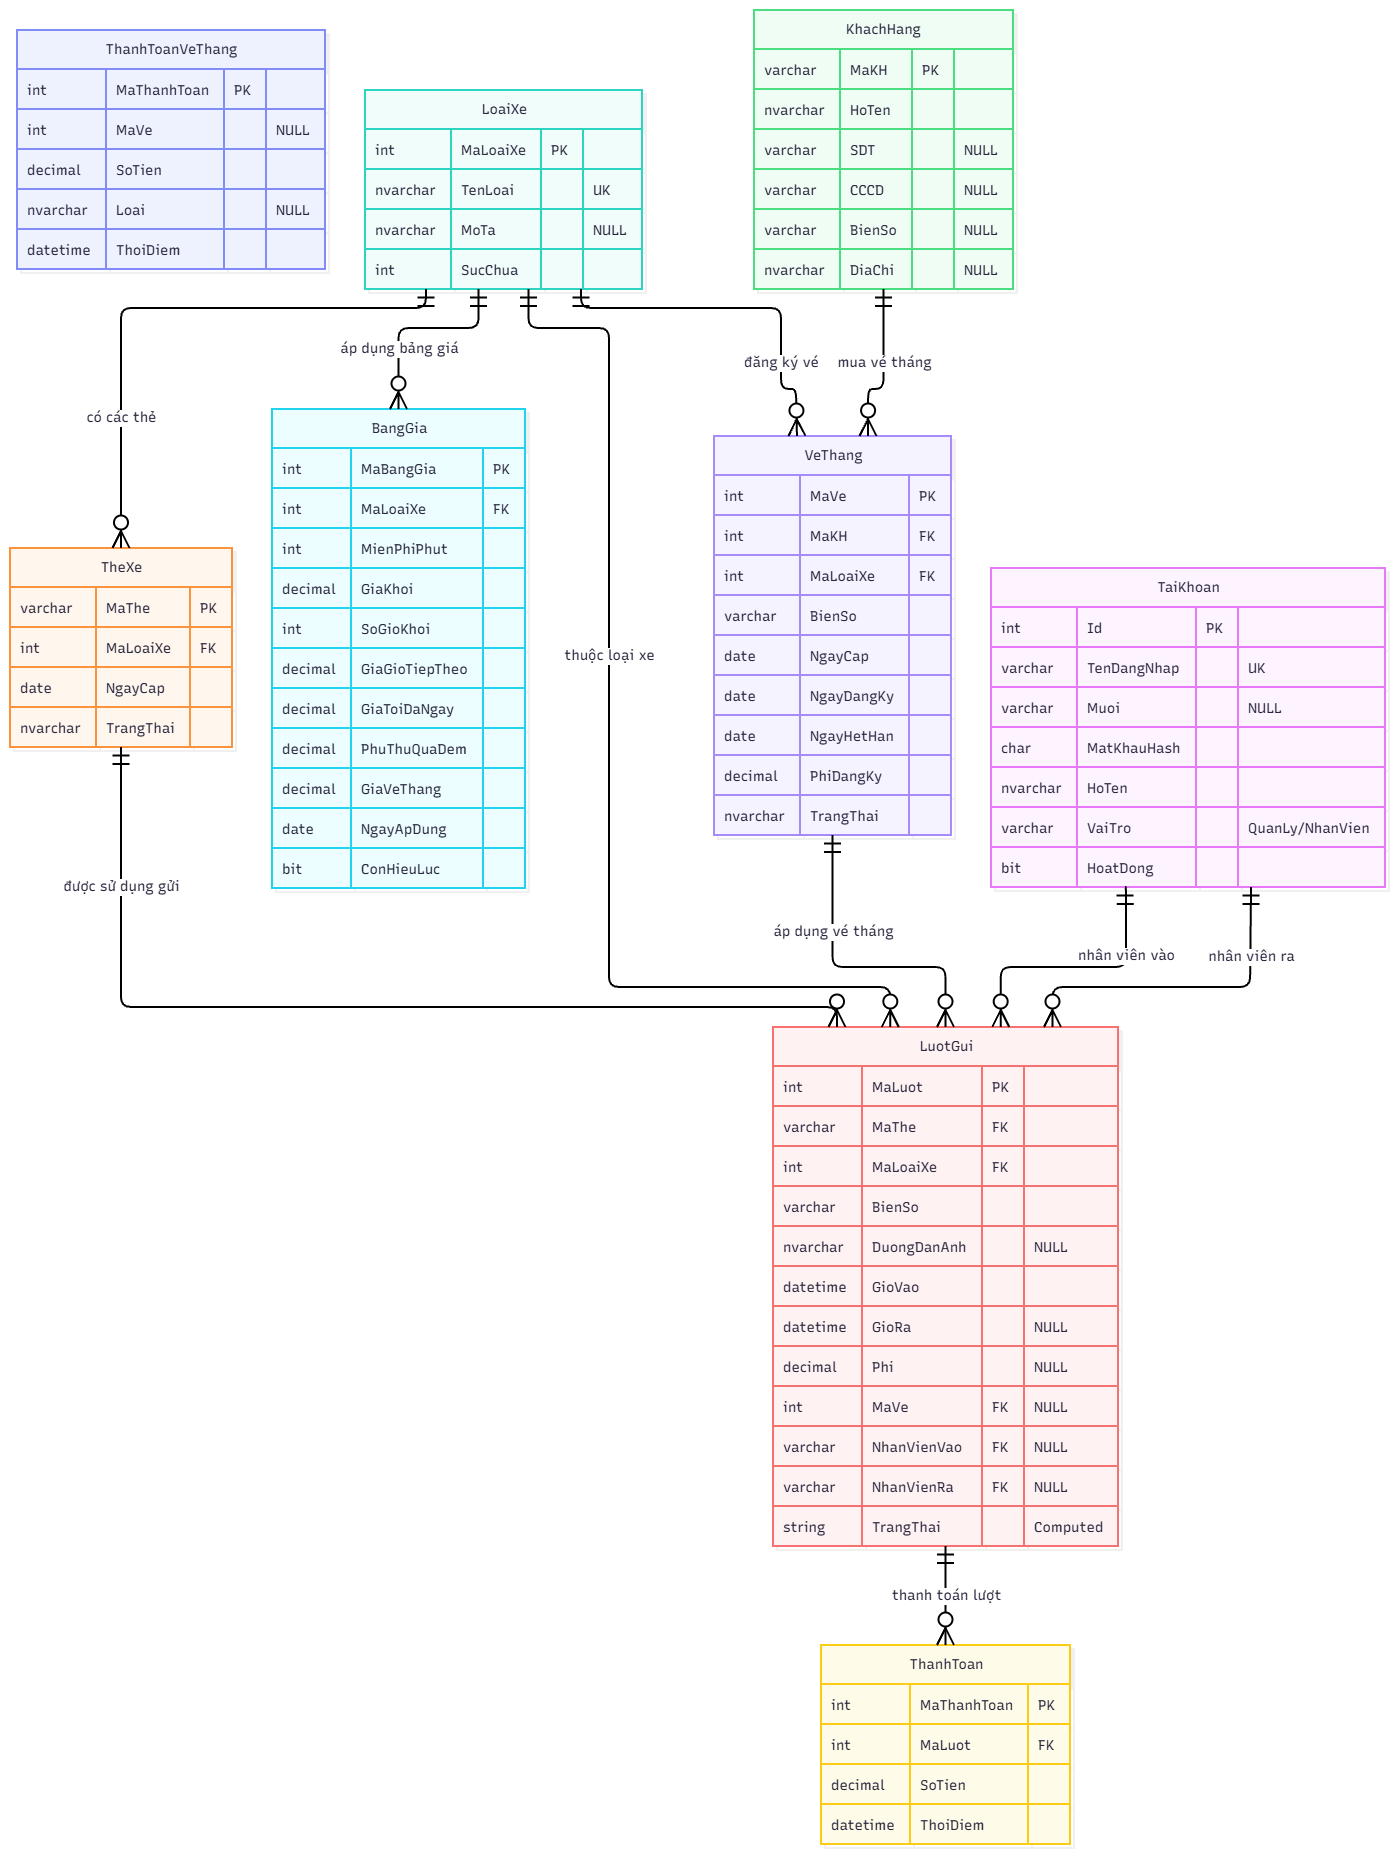
\includegraphics[width=\textwidth,height=0.6\textheight,keepaspectratio]{erd.png}
    \caption{Sơ đồ thực thể - liên kết của hệ thống}
    \label{fig:erd}
\end{figure}

% ==================================================
\section{Từ điển dữ liệu}
% ==================================================

\subsection{Bảng LoaiXe}

Bảng \texttt{LoaiXe} lưu thông tin các loại phương tiện được quản lý trong hệ thống.

\begin{table}[htbp]
    \centering
    \begin{tabular}{llll}
        \toprule
        \textbf{Tên cột} & \textbf{Kiểu dữ liệu} & \textbf{Ràng buộc} & \textbf{Mô tả} \\
        \midrule
        LoaiXeID   & INT          & PK       & Mã loại xe \\
        TenLoaiXe  & NVARCHAR(50) & NOT NULL & Tên loại xe \\
        \bottomrule
    \end{tabular}
    \caption{Từ điển dữ liệu bảng LoaiXe}
    \label{tab:loaixe}
\end{table}

\subsection{Bảng TheXe}

Bảng \texttt{TheXe} quản lý các thẻ xe được cấp phát tại bãi giữ xe.

\begin{table}[htbp]
    \centering
    \begin{tabular}{llll}
        \toprule
        \textbf{Tên cột} & \textbf{Kiểu dữ liệu} & \textbf{Ràng buộc} & \textbf{Mô tả} \\
        \midrule
        TheXeID  & INT         & PK     & Mã thẻ xe \\
        MaThe    & VARCHAR(20) & UNIQUE & Mã thẻ vật lý \\
        TrangThai & BIT        & NOT NULL & Trạng thái sử dụng \\
        \bottomrule
    \end{tabular}
    \caption{Từ điển dữ liệu bảng TheXe}
    \label{tab:thexe}
\end{table}

\subsection{Bảng KhachHang}

Bảng \texttt{KhachHang} lưu thông tin khách hàng đăng ký vé tháng.

\begin{table}[htbp]
    \centering
    \begin{tabular}{llll}
        \toprule
        \textbf{Tên cột} & \textbf{Kiểu dữ liệu} & \textbf{Ràng buộc} & \textbf{Mô tả} \\
        \midrule
        KhachHangID & INT          & PK       & Mã khách hàng \\
        HoTen       & NVARCHAR(100) & NOT NULL & Họ tên \\
        SoDienThoai & VARCHAR(20)  & NULL     & Số điện thoại \\
        BienSoXe    & VARCHAR(20)  & NULL     & Biển số xe \\
        \bottomrule
    \end{tabular}
    \caption{Từ điển dữ liệu bảng KhachHang}
    \label{tab:khachhang}
\end{table}

\subsection{Bảng VeThang}

Bảng \texttt{VeThang} lưu thông tin đăng ký vé tháng của khách hàng.

\begin{table}[htbp]
    \centering
    \begin{tabular}{llll}
        \toprule
        \textbf{Tên cột} & \textbf{Kiểu dữ liệu} & \textbf{Ràng buộc} & \textbf{Mô tả} \\
        \midrule
        VeThangID   & INT  & PK & Mã vé tháng \\
        KhachHangID & INT  & FK & Khách hàng sở hữu \\
        TheXeID     & INT  & FK & Thẻ xe được cấp \\
        NgayBatDau  & DATE & NOT NULL & Ngày bắt đầu \\
        NgayHetHan  & DATE & NOT NULL & Ngày hết hạn \\
        \bottomrule
    \end{tabular}
    \caption{Từ điển dữ liệu bảng VeThang}
    \label{tab:vethang}
\end{table}

\subsection{Bảng LuotGui}

Bảng \texttt{LuotGui} lưu thông tin của từng lượt gửi xe phát sinh tại bãi.

\begin{table}[htbp]
    \centering
    \begin{tabular}{llll}
        \toprule
        \textbf{Tên cột} & \textbf{Kiểu dữ liệu} & \textbf{Ràng buộc} & \textbf{Mô tả} \\
        \midrule
        LuotGuiID & INT           & PK       & Mã lượt gửi \\
        TheXeID   & INT           & FK       & Thẻ xe sử dụng \\
        LoaiXeID  & INT           & FK       & Loại xe \\
        BienSoXe  & VARCHAR(20)   & NOT NULL & Biển số xe \\
        GioVao    & DATETIME      & NOT NULL & Giờ vào bãi \\
        GioRa     & DATETIME      & NULL     & Giờ ra bãi \\
        PhiGuiXe  & DECIMAL(18,0) & NULL     & Phí gửi xe \\
        \bottomrule
    \end{tabular}
    \caption{Từ điển dữ liệu bảng LuotGui}
    \label{tab:luotgui}
\end{table}

\subsection{Bảng BangGia}

Bảng \texttt{BangGia} lưu thông tin đơn giá áp dụng cho từng loại xe
trong hệ thống. Việc tách bảng giá thành một thực thể riêng giúp
người quản lý có thể thay đổi chính sách giá mà không ảnh hưởng tới
dữ liệu lịch sử của các lượt gửi xe đã phát sinh.

Mỗi bản ghi trong bảng tương ứng với một loại xe và mức giá được
áp dụng. Trong tương lai, thiết kế này cũng cho phép mở rộng thêm
các loại giá khác nhau như giá theo giờ, giá theo ngày hoặc giá
vé tháng.

\paragraph{Ràng buộc dữ liệu}

\begin{itemize}
    \item BangGiaID là khóa chính của bảng.

    \item LoaiXeID là khóa ngoại tham chiếu đến bảng LoaiXe.

    \item Đơn giá phải lớn hơn 0.

    \item Mỗi loại xe phải được gắn với ít nhất một mức giá hợp lệ.
\end{itemize}


% ==================================================
\section{Sơ đồ tuần tự}
% ==================================================

\subsection{Nghiệp vụ xe vào}

Nghiệp vụ xe vào được thực hiện theo trình tự sau:

\begin{enumerate}
    \item Nhân viên nhập biển số xe và chọn loại xe.
    \item Hệ thống kiểm tra trạng thái thẻ xe.
    \item Hệ thống tạo lượt gửi mới.
    \item Hệ thống lưu thời điểm vào bằng giờ hệ thống.
    \item Hệ thống cập nhật trạng thái thẻ.
    \item Hệ thống in vé xe.
\end{enumerate}

% Hình sơ đồ tuần tự xe vào sẽ được chèn vào đây
% \begin{figure}[htbp]
%     \centering
%     \includegraphics[width=\textwidth]{seq-xevao.png}
%     \caption{Sơ đồ tuần tự nghiệp vụ xe vào}
%     \label{fig:seq-xevao}
% \end{figure}

\subsection{Nghiệp vụ xe ra và thanh toán}

Đây là nghiệp vụ quan trọng nhất của hệ thống vì liên quan trực tiếp đến tính phí và doanh thu. Quy trình xử lý diễn ra như sau:

\begin{enumerate}
    \item Nhân viên nhập mã thẻ xe hoặc biển số xe.
    \item Hệ thống tìm lượt gửi đang hoạt động.
    \item Hệ thống ghi nhận thời gian xe ra.
    \item Hệ thống kiểm tra tình trạng vé tháng.
    \item Hệ thống tính phí gửi xe.
    \item Nhân viên xác nhận thanh toán.
    \item Hệ thống thực hiện transaction bao gồm:
    \begin{itemize}
        \item Cập nhật giờ ra.
        \item Lưu số tiền thanh toán.
        \item Giải phóng thẻ xe.
    \end{itemize}
    \item Hệ thống in biên nhận.
\end{enumerate}

Nếu xảy ra lỗi trong quá trình ghi dữ liệu, transaction sẽ bị hủy và cơ sở dữ liệu được khôi phục về trạng thái trước đó.

% Hình sơ đồ tuần tự xe ra sẽ được chèn vào đây
% \begin{figure}[htbp]
%     \centering
%     \includegraphics[width=\textwidth]{seq-xera.png}
%     \caption{Sơ đồ tuần tự nghiệp vụ xe ra và thanh toán}
%     \label{fig:seq-xera}
% \end{figure}

% ==================================================
\section{Thiết kế giao diện}
% ==================================================

Các giao diện được thiết kế theo nguyên tắc đơn giản, trực quan và giảm tối đa số thao tác của nhân viên tại cổng xe.

Các màn hình chính gồm:

\begin{itemize}
    \item Giao diện đăng nhập.
    \item Giao diện ghi nhận xe vào.
    \item Giao diện ghi nhận xe ra.
    \item Giao diện quản lý vé tháng.
    \item Giao diện quản lý loại xe và bảng giá.
    \item Giao diện quản lý thẻ xe.
    \item Giao diện tra cứu lịch sử.
    \item Giao diện thống kê doanh thu.
\end{itemize}

Đối với các màn hình nghiệp vụ xe vào và xe ra, các trường thông tin quan trọng được đặt ở vị trí trung tâm để thuận tiện cho việc thao tác nhanh tại cổng.

Các bảng dữ liệu sử dụng điều khiển \texttt{DataGridView} nhằm hỗ trợ hiển thị, tìm kiếm và cập nhật dữ liệu hiệu quả.

Phần thiết kế giao diện chỉ mô tả cấu trúc và bố cục tổng quát. Các ảnh chụp giao diện thực tế sau khi triển khai sẽ được trình bày trong Chương~5.

% ==================================================
\section{Tóm tắt chương}
% ==================================================

Chương này đã trình bày thiết kế tổng thể của hệ thống quản lý bãi giữ xe, bao gồm kiến trúc ba lớp, mô hình dữ liệu, từ điển dữ liệu và các luồng xử lý nghiệp vụ chính.

Kết quả thiết kế là cơ sở để triển khai hệ thống bằng ngôn ngữ C\#, Windows Forms và SQL Server trong chương tiếp theo.
